
\section{Résultats obtenus et analyse}
 
\subsection{Résultats de différents scénarios}

\subsubsection{Variation de taille d'apprentissage}
Comme nous travaillons sur des séries temporelles, qui ne sont pas stationnaires, nous nous intéressons à l'effet de la taille d'apprentissage sur la précision de la prédiction du rendement de l'action. Nous avons réalisé des tests sur l'action Renault dans l'indice CAC40.\\

Sur la figure \ref{fig:SE_Trainingset}, nous observons un très grand pic au début d'octobre 2008 avec une taille d'apprentissage de 120 jours (6 mois), juste après le début de la crise mi-septembre. Toutefois, ce pic est absent sur les autres courbes. Cela signifie que notre modèle est capable de détecter le début de la période de la crise, puisqu'une fois que celle-ci est arrivée, la tendance du marché est brutalement rompue. Dans ce cas, apprendre sur les données des 6 derniers mois n'est pas une bonne approche pour la prédiction du rendement. En revanche, apprendre sur une période plus courte est plus efficace pour ne prendre en compte que les informations intéressantes de l'évolution du marché.\\

Dans les autres périodes, nous pouvons constater que l'erreur quadratique de la prédiction du rendement est proche de zéro dans les quatre cas.

\begin{figure}[H]
\centering
\begin{subfigure}{.5\textwidth}
\centering
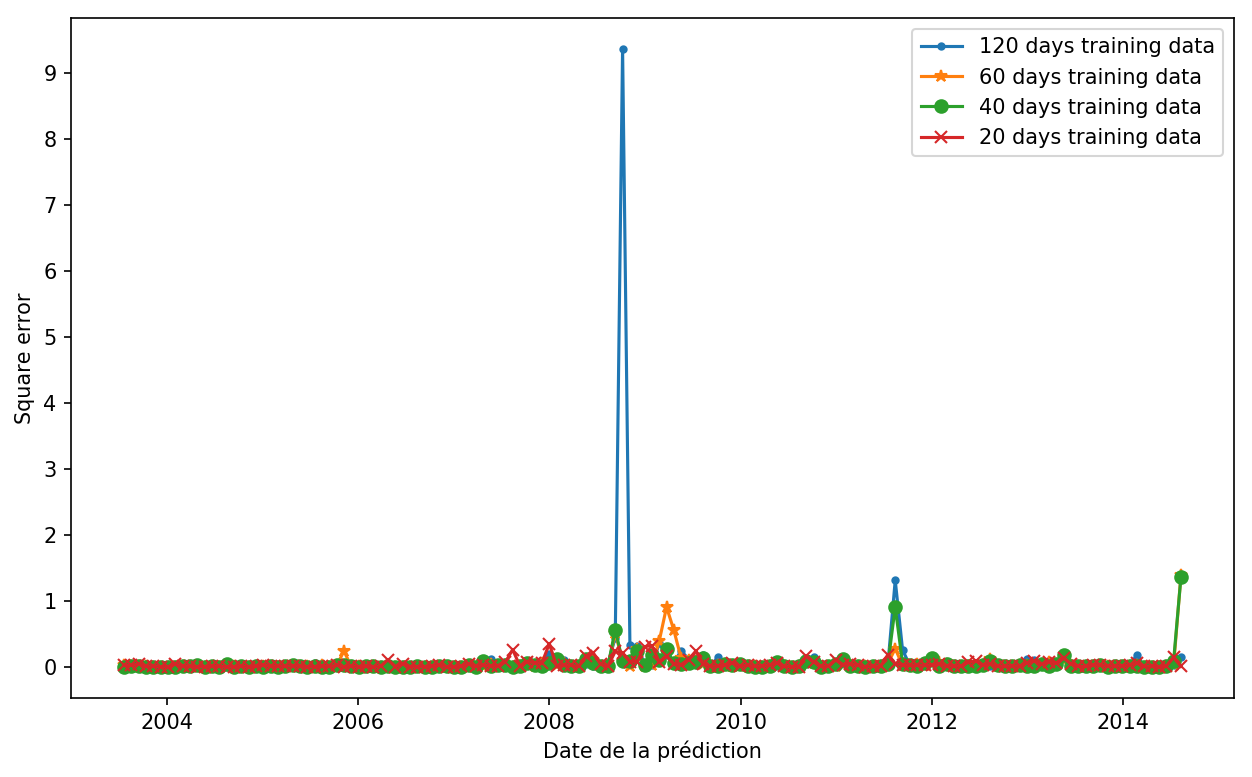
\includegraphics[width=.9\linewidth, scale=0.2]
{plot/SE_Trainingset.png}
\caption{Vue globale sur 10 ans}
\label{fig:SE_Ts1}
\end{subfigure}%
\begin{subfigure}{.5\textwidth}
\centering
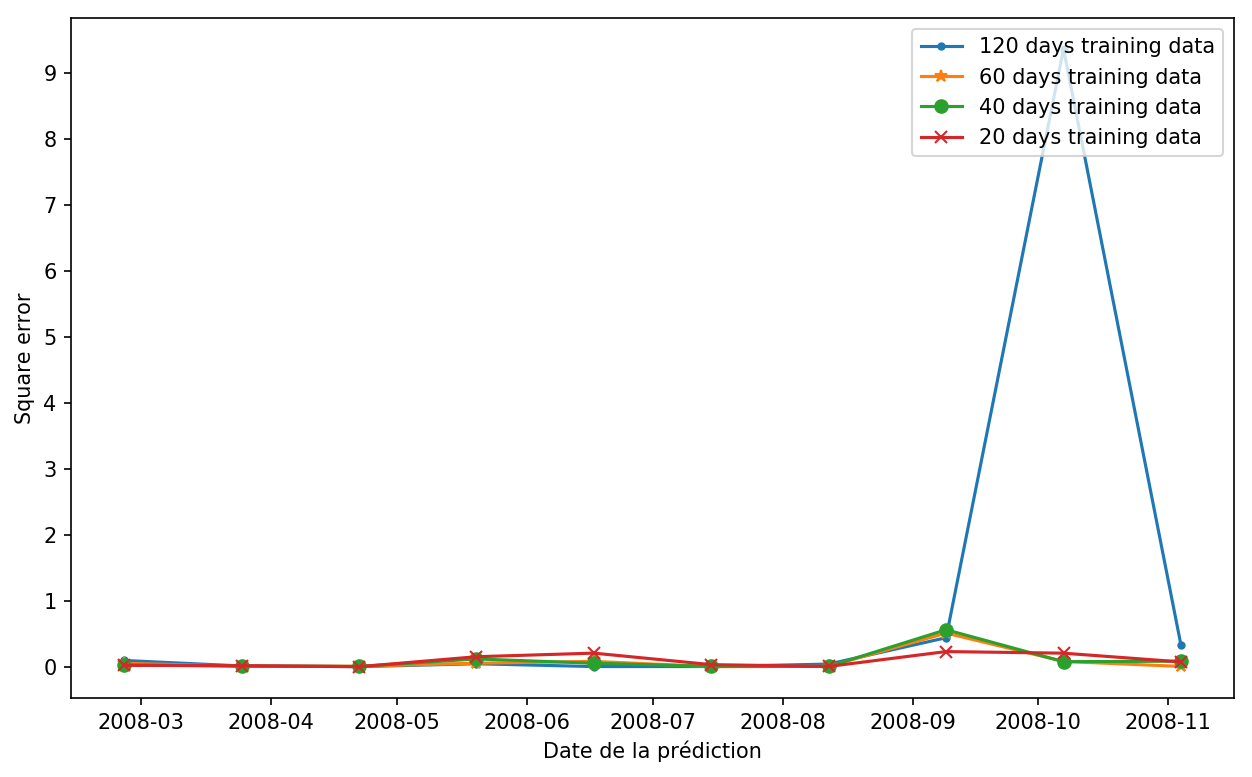
\includegraphics[width=.9\linewidth, scale=0.2]
{plot/SE_Trainingset_s.png}
\caption{Vue zoomée sur la période de la crise de 2008}
\label{fig:SE_Ts2}
\end{subfigure}
\caption{Erreur quadratique de la prédiction du rendement de Renault à un horizon de 20 jours (1 mois) en fonction de la taille d'apprentissage}
\label{fig:SE_Trainingset}
\end{figure}

En observant les figures ci-dessous, nous remarquons que l'erreur moyenne pour 120 jours est généralement plus petite que les autres cas (sauf la période de la crise), car une periode plus longue contient plus d'informations et peut mieux présenter la tendance du marché. Au contraire, une période plus courte est plus bruitée.

\begin{figure}[H]
\centering
\begin{subfigure}{.5\textwidth}
\centering
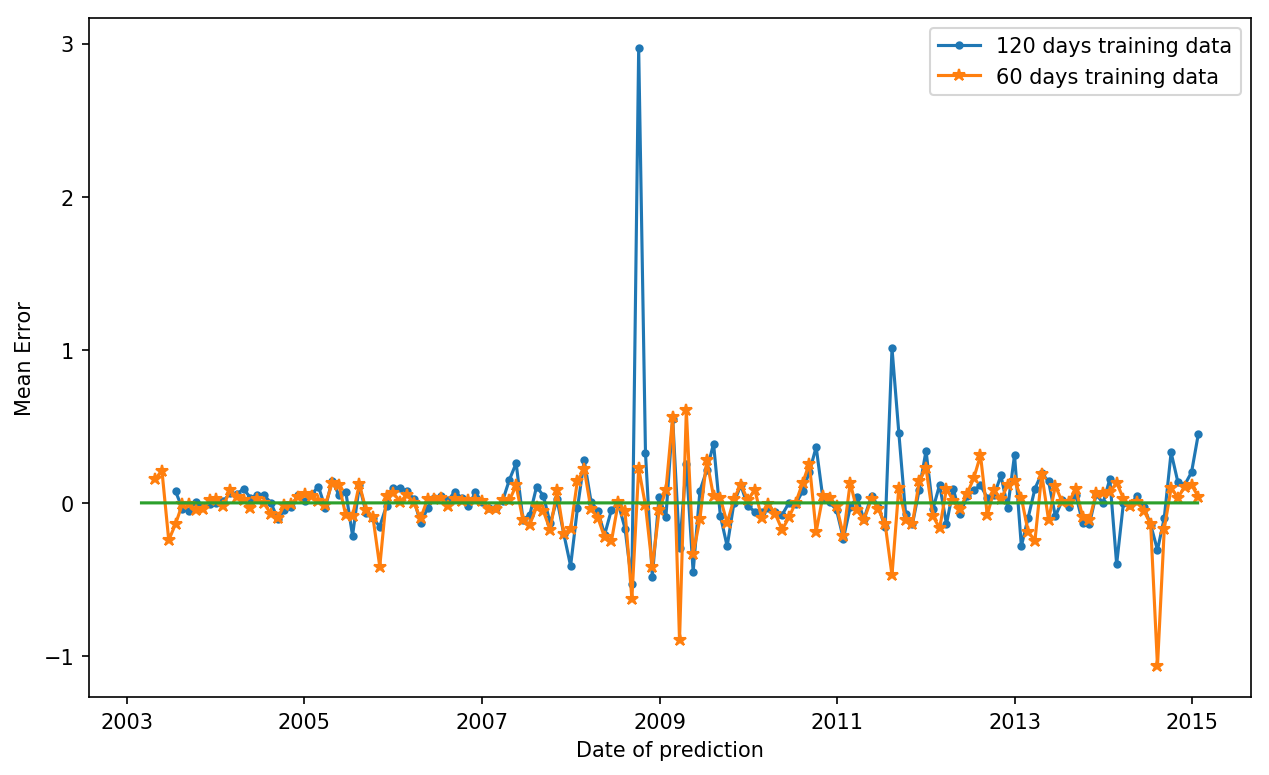
\includegraphics[width=.9\linewidth, scale=0.2]
{plot/ME_Trainingset1.png}
\caption{Erreur moyenne pour 120 et 60 jours}
\label{fig:ME_Ts1}
\end{subfigure}%
\begin{subfigure}{.5\textwidth}
\centering
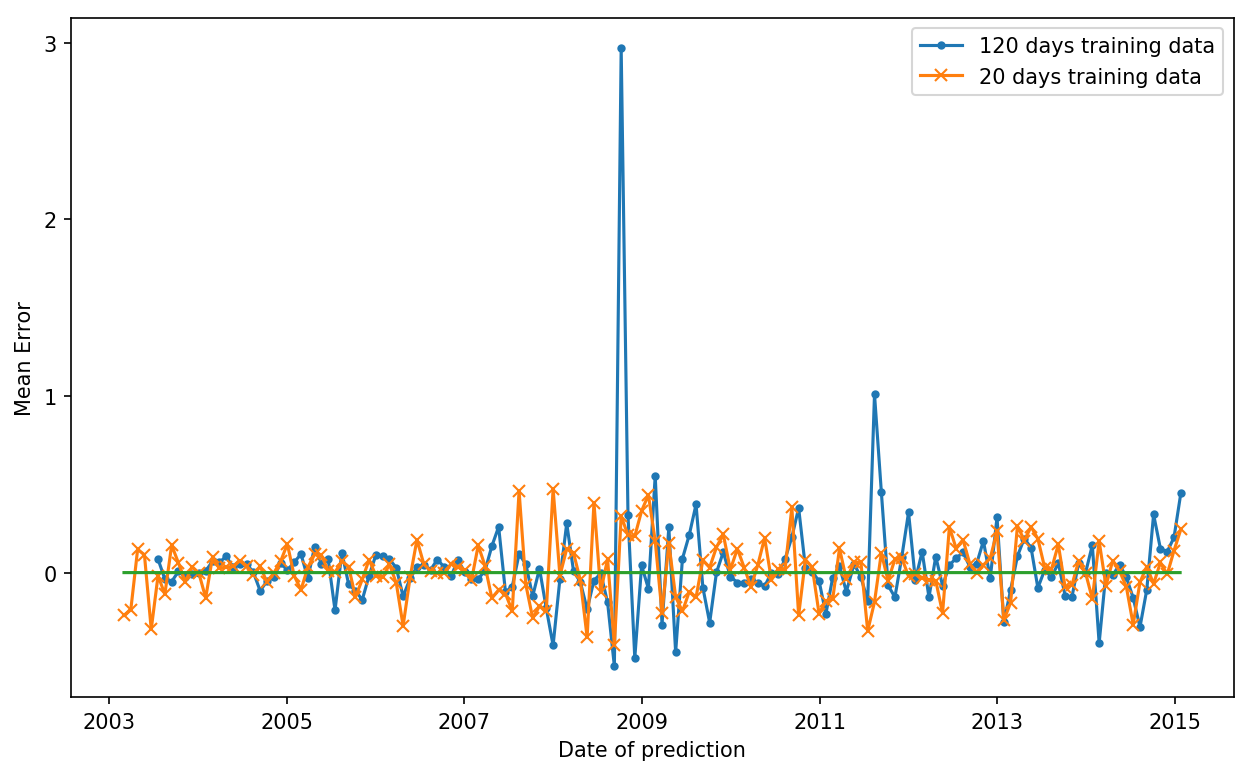
\includegraphics[width=.9\linewidth, scale=0.2]
{plot/ME_Trainingset2.png}
\caption{Erreur moyenne pour 120 et 20 jours}
\label{fig:ME_Ts2}
\end{subfigure}
\caption{Erreur Moyenne de la prédiction du rendement de Renault à un horizon de 20 jours (1 mois) en fonction de la taille d'apprentissage}
\label{fig:ME_Trainingset}
\end{figure}


\subsubsection{Variation de l'horizon}

Nous discutons l'influence de l'horizon de prédiction dans cette partie, pour déterminer la fréquence de la gestion d'un portefeuille, il faut bien choisir un horizon de prédiction. Si nous prenons un horizon très court, ça va générer un coût opérationel très élevé, parce que nous avons besoin de prendre plus de temps et plus de ressources. Par contre, si nous définissons un horizon plus long, il est plus difficile de prédire la valeur très future, donc ça va dégrader la performance du modèle. \\

Nous avons fixé la taille de base d'apprentissage à 120j (6 mois) et la taille de base de test à 20j (1 mois), nous avons pris tout les 13 TIs, nous n'avons changé que l'horizon de prédiction. Nous avons préparé 6 tests pour savoir l'influence des horizons différents, nous avons varié l'horizon sur 5j (1 semaine), 10j (2 semaines), 20j (1 mois), 40j (2 mois), 60j (3 mois), 120j (6 mois). \\

Nous pouvons obtenir le résultat global sur 15 ans dans la figure \ref{fig:Horizon}. Suivi l'augementation de l'horizon, nous pouvons constater que la prériode défavorable est plus fluctuante et il y a plus de pics sur la courbe. Pendant la période stable, les erreurs moyennes quadratiques sont plus proche de zéro quand l'horizon est plus petit. En comparant avec l'évolution du prix d'action Renault, nous avons trouvé que quand il y a une baisse évidente, les erreure de prédictions sont aussi plus grandes. \\

Sur la figure \ref{fig:Prix_action}, il y a 5 baisses plus évidentes sur la courbe, elles sont dans le septembre 2001, le mars 2003, le septembre 2008, l'octobre 2011 et le novembre 2014. A la suite des événements du 11 septembre 2001, Renault atteint le 21 septembre son point bas de l'année à 26,01 euros.[2001] Le titre Renault connaît un plus bas le 12 mars 2003 à 29,51 euros, suivant le mouvement de baisse du secteur automobile, pénalisé par les incertitudes économiques et géopolitiques et affecté par le recul des performances commerciales du début d’année.[2003] Le septembre 2008 est la crise financière mondiale. ...[2011] Renault a accusé une baisse globale de 5 pourcents de ses ventes en novembre 2014. [2014] Pendant ces périodes défavorables, la situstion est plus pire, les erreurs de prédictions sont plus grandes. Quand l'horizon est plus long, la courbe est plus perturpée. \\ 



\begin{figure}[H]
	\centering
	\begin{subfigure}{.5\textwidth}
	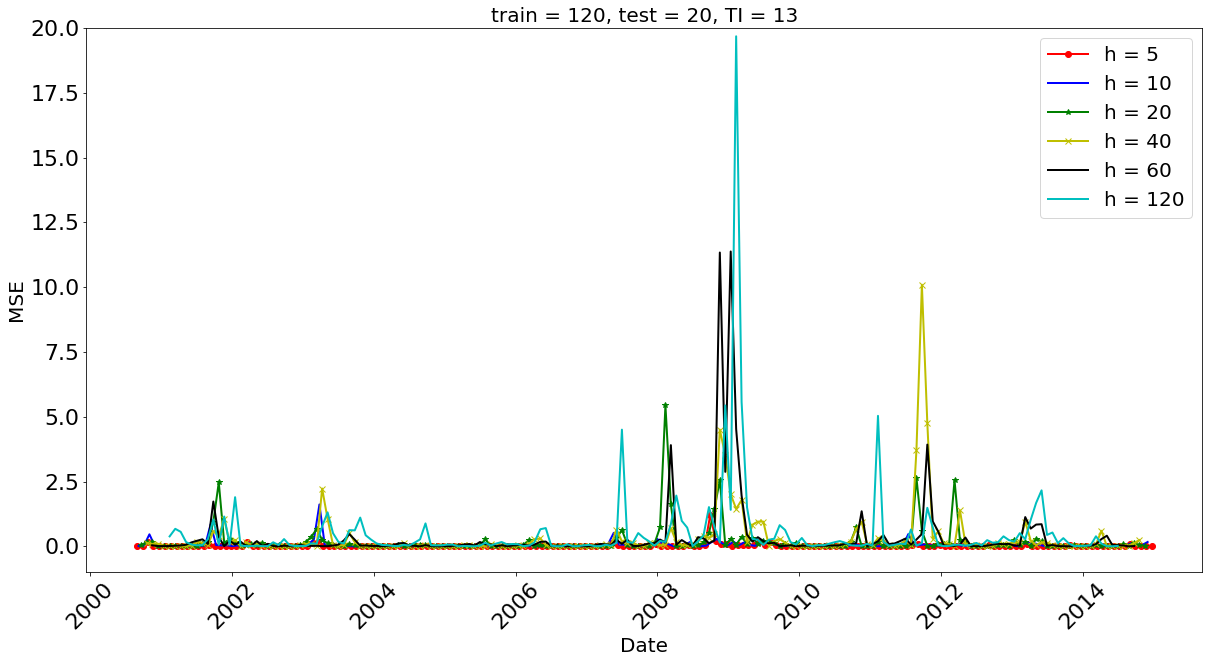
\includegraphics[width=.9\linewidth, scale=0.2]
	{plot/MSE_120_h_20.png}
	\caption{MSE en fonction de la variation de l'horizon}
	\label{fig:Horizon}
	\end{subfigure}%
	\begin{subfigure}{.5\textwidth}
	\centering
	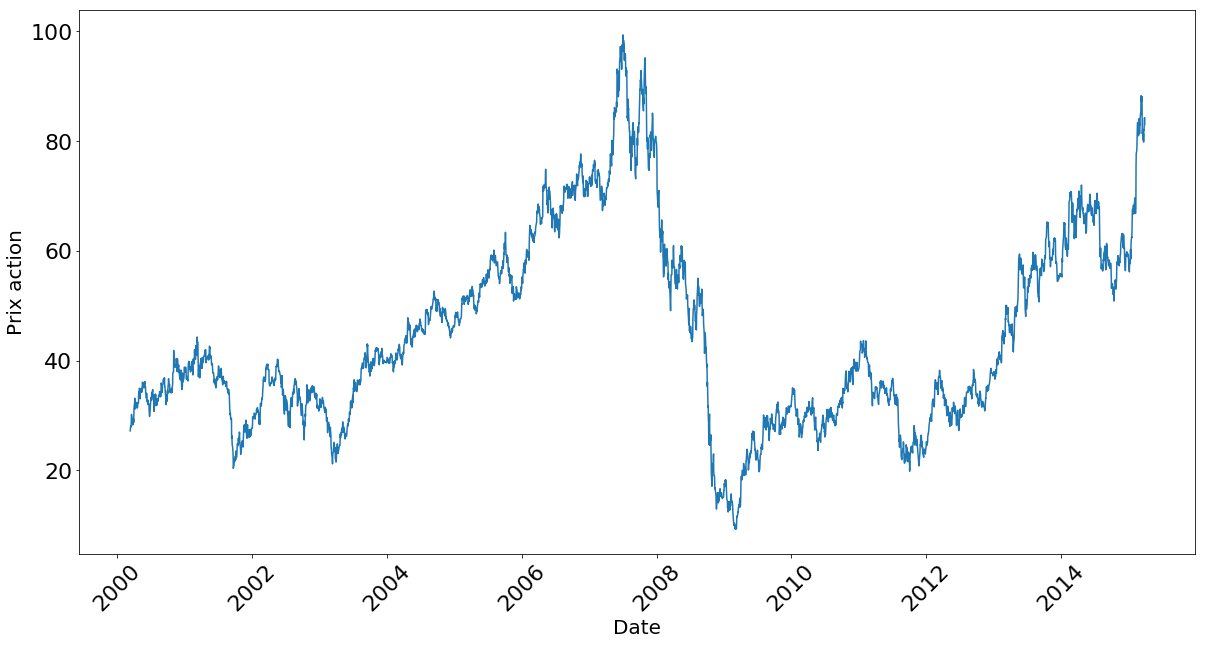
\includegraphics[width=.9\linewidth, scale=0.2]
	{plot/Prix_action_global.png}
	\caption{L'évolution du Prix d'action Renault}
	\label{fig:Prix_action}
	\end{subfigure}
\caption{L'influence de l'horizon sur en vue global pendant 2000 - 2015}
\label{fig:ME_Trainingset}
\end{figure}

Pour comparer l'impact de l'horizon sur les périodes différentes, nous avons aussi fait un zoom sur la période autour de la crise financière de 2008, les figures ci-après vous montre nos résultat. La figure \ref{fig:Prix_crise} est le prix d'action entre 2007 et 2010, nous pouvons trouver qu'à partir du septembre 2007, la courbe commence à baisser progressivement et elle apparait une chute au septembre 2008. Après mars 2009, le prix d'action commence à revenir. La figure \ref{fig:Horizon_crise} nous montre que pendant la crise toutes les prédictions ne sont pas stables, il y a une erreur de prédiction sur chaque courbe. Par contre, quand l'horizon est plus long, il y a un retard de détection sur la tendance de baisse. Quand l'horizon est 20, ses pics sont plus proche au début de la baisse de cours, pour l'horizon est égale à 60 et 120, il y a toujours un décalage avec la date début. Les figures \ref{fig:Horizon_before} et \ref{fig:Horizon_after} sont les prériodes avant et après la crise de 2008, nous pouvons consatater que les erreurs sont négligables par rapports à la prériode de crise. Mais, l'horizon est plus grand, la courbe est plus fluctuante.

\begin{figure}[H]
	\centering
	\begin{subfigure}{.5\textwidth}
	\centering
	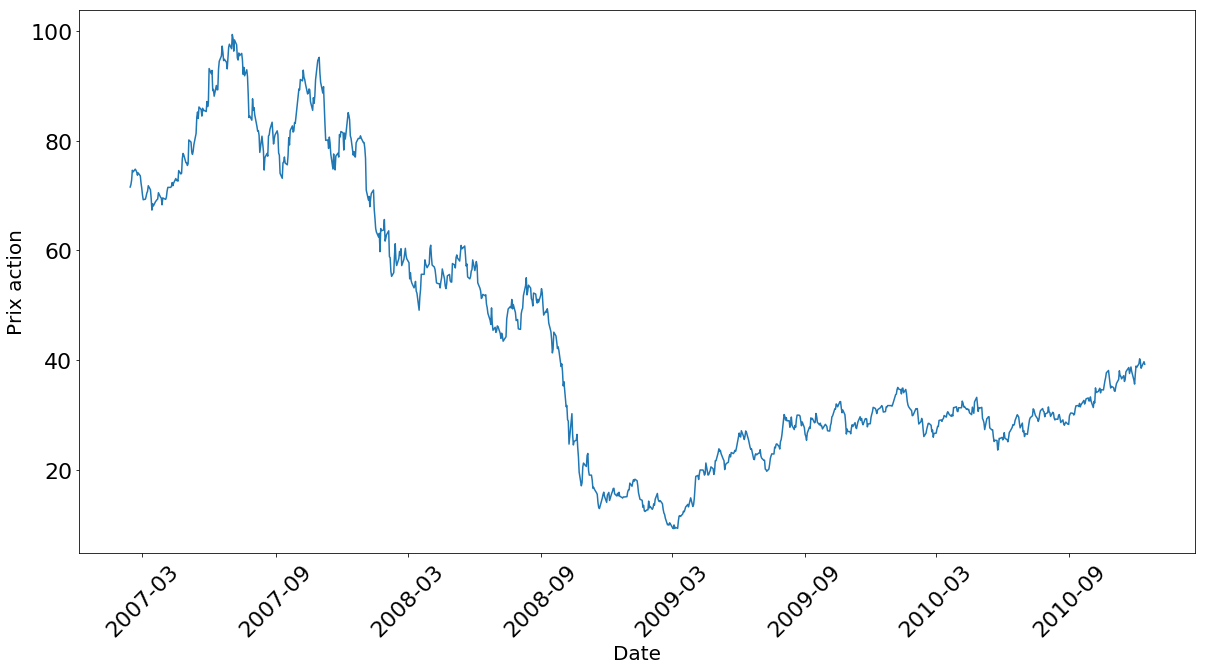
\includegraphics[width=.9\linewidth, scale=0.2]
	{plot/Prix_action_crise.png}
	\caption{Prix d'action pendant la crise 2008}
	\label{fig:Prix_crise}
	\end{subfigure}%
	\begin{subfigure}{.5\textwidth}
	\centering
	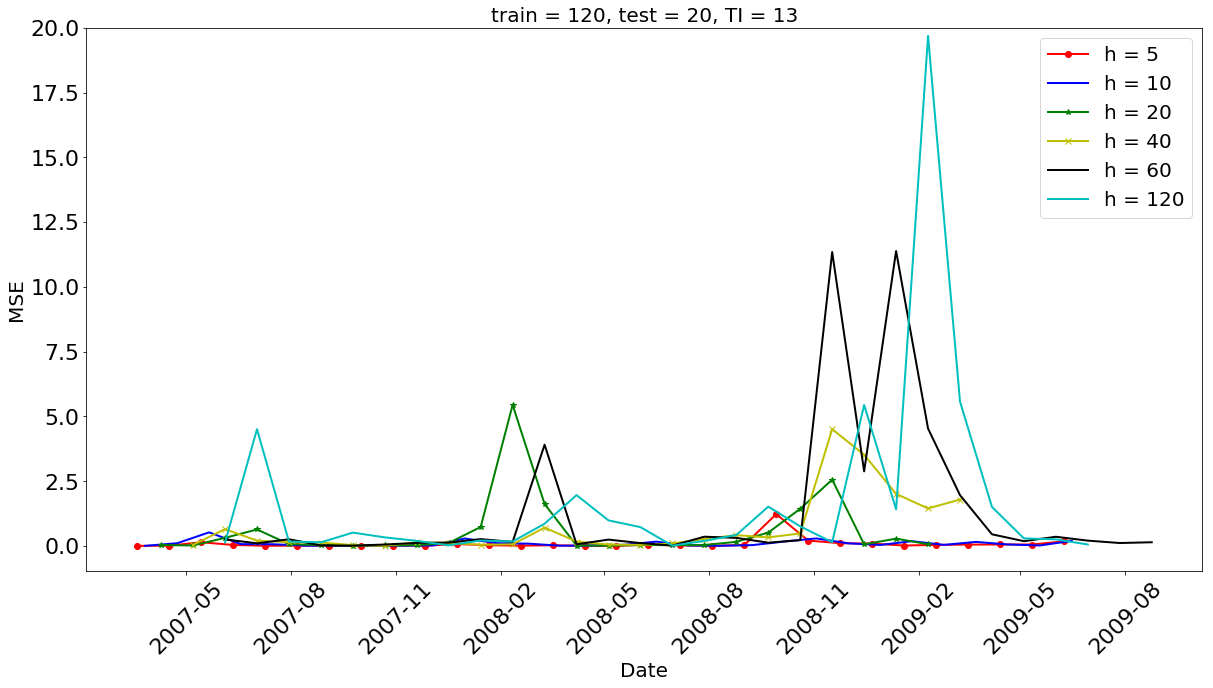
\includegraphics[width=.9\linewidth, scale=0.2]
	{plot/MSE_120_h_20_crise.png}
	\caption{MSE pendant la crise 2008}
	\label{fig:Horizon_crise}
	\end{subfigure} 
	\begin{subfigure}{.5\textwidth}
	\centering
	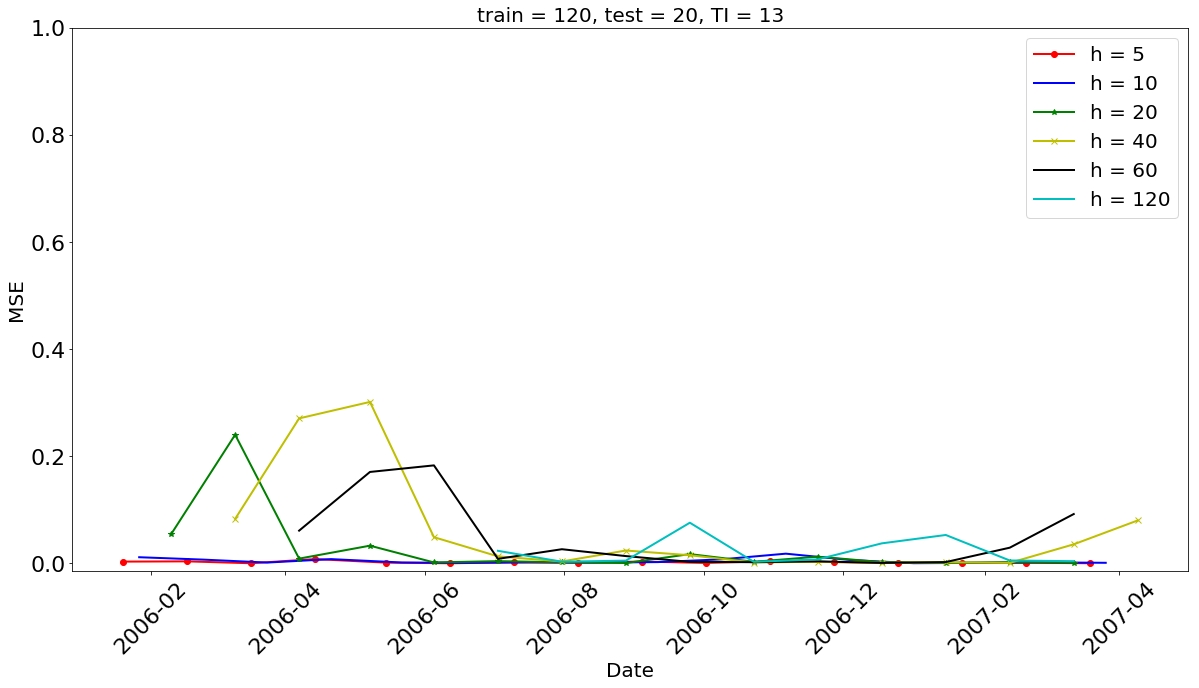
\includegraphics[width=.9\linewidth, scale=0.2]
	{plot/MSE_120_h_20_before.png}
	\caption{MSE avant la crise 2008}
	\label{fig:Horizon_before}
	\end{subfigure}%
	\begin{subfigure}{.5\textwidth}
	\centering
	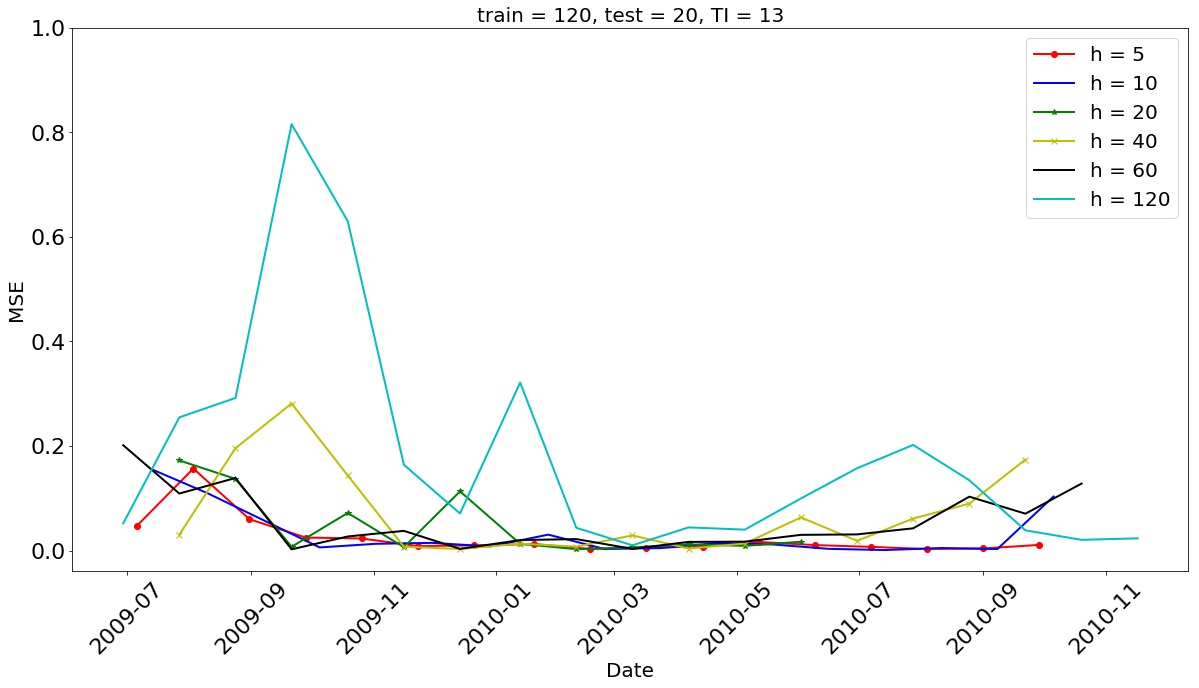
\includegraphics[width=.9\linewidth, scale=0.2]
	{plot/MSE_120_h_20_after.png}
	\caption{MSE après la crise 2008}
	\label{fig:Horizon_after}
	\end{subfigure}
\caption{L'influence de l'horizon sur les prériodes différentes}
\label{fig:ME_Trainingset}
\end{figure}


\subsection{Evaluation du modèle}

MSE : $ E((V_{true} - V_{pred})^2) $

\subsection{Difficultés rencontrées}


L’apprentissage a pris trop de temps.

Trop de scénarios

Bcp d’actions
